\documentclass{beamer}
\mode<presentation>
\usepackage{amsmath}
\usepackage{amssymb}
%\usepackage{advdate}
\usepackage{adjustbox}
\usepackage{subcaption}
\usepackage{enumitem}
\usepackage{multicol}
\usepackage{mathtools}
\usepackage{listings}
\usepackage{url}
\def\UrlBreaks{\do\/\do-}
\usetheme{Boadilla}
\usecolortheme{lily}
\setbeamertemplate{footline}
{
  \leavevmode%
  \hbox{%
  \begin{beamercolorbox}[wd=\paperwidth,ht=2.25ex,dp=1ex,right]{author in head/foot}%
    \insertframenumber{} / \inserttotalframenumber\hspace*{2ex} 
  \end{beamercolorbox}}%
  \vskip0pt%
}
\setbeamertemplate{navigation symbols}{}

\providecommand{\nCr}[2]{\,^{#1}C_{#2}} % nCr
\providecommand{\nPr}[2]{\,^{#1}P_{#2}} % nPr
\providecommand{\mbf}{\mathbf}
\providecommand{\pr}[1]{\ensuremath{\Pr\left(#1\right)}}
\providecommand{\qfunc}[1]{\ensuremath{Q\left(#1\right)}}
\providecommand{\sbrak}[1]{\ensuremath{{}\left[#1\right]}}
\providecommand{\lsbrak}[1]{\ensuremath{{}\left[#1\right.}}
\providecommand{\rsbrak}[1]{\ensuremath{{}\left.#1\right]}}
\providecommand{\brak}[1]{\ensuremath{\left(#1\right)}}
\providecommand{\lbrak}[1]{\ensuremath{\left(#1\right.}}
\providecommand{\rbrak}[1]{\ensuremath{\left.#1\right)}}
\providecommand{\cbrak}[1]{\ensuremath{\left\{#1\right\}}}
\providecommand{\lcbrak}[1]{\ensuremath{\left\{#1\right.}}
\providecommand{\rcbrak}[1]{\ensuremath{\left.#1\right\}}}
\theoremstyle{remark}
\newtheorem{rem}{Remark}
\newcommand{\sgn}{\mathop{\mathrm{sgn}}}
\providecommand{\abs}[1]{\left\vert#1\right\vert}
\providecommand{\res}[1]{\Res\displaylimits_{#1}} 
\providecommand{\norm}[1]{\lVert#1\rVert}
\providecommand{\mtx}[1]{\mathbf{#1}}
\providecommand{\mean}[1]{E\left[ #1 \right]}
\providecommand{\fourier}{\overset{\mathcal{F}}{ \rightleftharpoons}}
%\providecommand{\hilbert}{\overset{\mathcal{H}}{ \rightleftharpoons}}
\providecommand{\system}{\overset{\mathcal{H}}{ \longleftrightarrow}}
	%\newcommand{\solution}[2]{\textbf{Solution:}{#1}}
%\newcommand{\solution}{\noindent \textbf{Solution: }}
\providecommand{\dec}[2]{\ensuremath{\overset{#1}{\underset{#2}{\gtrless}}}}
\newcommand{\myvec}[1]{\ensuremath{\begin{pmatrix}#1\end{pmatrix}}}
\let\vec\mathbf

\lstset{
%language=C,
frame=single, 
breaklines=true,
columns=fullflexible
}

\numberwithin{equation}{section}

\title{Area between two curves by using matrix method}
\author{Deepak Ahirwar  \\ Electrical Enggineering ,\\IIT Hyderabad.}

\date{\today} 
\begin{document} 

\begin{frame}
\titlepage
\end{frame}

\section*{Outline}
\begin{frame}
\tableofcontents
\end{frame}
\section{Problem}
\begin{frame}
\frametitle{Problem Statement}

Find the area of the circle $ 4x^2 + 4y^2 = 9$ which is interior to the parabola $x^2 = 4y.$
\\ \begin{table}[h!]    
  \centering
  \begin{tabular}[12pt]{ |c| c|}
    \hline
    \textbf{Variable} & \textbf{Description}\\ 
    \hline
    $V_1,u_1,f_1$ & Parameters of Parabola \\
    \hline 
    $V_2,u_2,f_2$ & Parameters of circle \\
    \hline
     $P_1,P_2$ & Points of intersection \\
     \hline
     $A$ & Area between the conics \\
    \hline
\end{tabular}

  \caption{Variables Used}
\end{table}

\end{frame}

%\subsection{Literature}
\section{Solution}
\subsection{Conic Parameters}
\begin{frame}
\frametitle{Conic Parameters}
%\framesubtitle{Literature}
 The conic parameters of circle $4x^2+4y^2=9$ are :
 \begin{center}
      $V_1 = \myvec{ 1 &0\\ 0 &1}, u_1 =\myvec{0 \\ 0}, f_1 = -\frac{9}{4} $
 \end{center}
 Conic parameters of parabola $x^2=4y$ can be expressed as :
 \begin{center}
      $V_2 = \myvec{ 1 &0\\ 0 &0}, u_2 =\myvec{0 \\ -2}, f_2 = 0$
 \end{center}
 
\end{frame}

\subsection{Intersection of conics}
\begin{frame}
\frametitle{Intersection of conics}
The intersection of two conics with parameters$ V_i, u_i, f_i (i = 1, 2) $is defined as :
\begin{center}
    $x^\top (V_1 + \mu V_2) x + 2(u_1 + \mu u_2)^\top x + (f_1 + \mu f_2) = 0$
\end{center}

On solving we get the points of intersection are :
\begin{center}
    $\myvec{\sqrt{2}\\\frac{1}{2}}\;,\myvec{-\sqrt{2}\\\frac{1}{2}}$
\end{center}

\end{frame}
\subsection{Area calculation}
\begin{frame}
\frametitle{Area calculation}
Area between the curves is,
\begin{align}
2\int_{0}^{\frac{1}{2}} \brak{\sqrt{\frac{9}{4}-y^2}-\sqrt{4y}} \, dy 
\end{align}
By solving the integration, we get area is equal to 3.005 sq.units
\end{frame}

\subsection{Figure}
\begin{frame}
\frametitle{Figure}

\begin{figre}[h!]
   \centering
   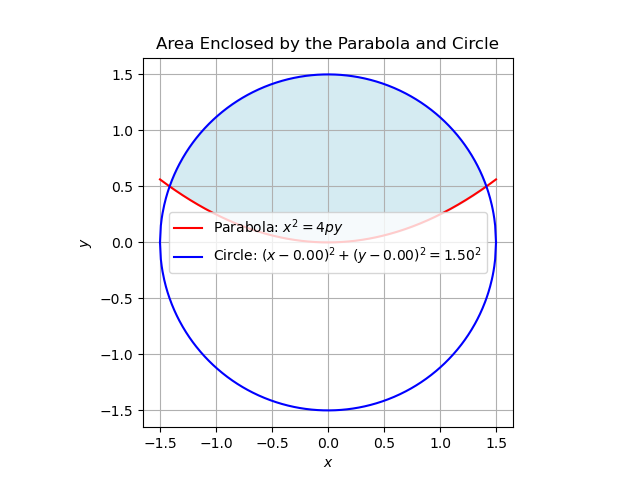
\includegraphics[width=\linewidth]{figs/fig2.png}
   \label{stemplot}
   \caption{}
\end{figure}
    
\end{frame}

\section{C Code}
\begin{frame}[fragile]
\frametitle{C Code for generating points on line}
\begin{lstlisting}[language=C]
#include <stdio.h>

int main() {
    // Define parabola and circle parameters
    // Parabola equation: x^2 = 4py, so y = x^2 / (4 * p)
    double p = 1.0; // Parabola parameter (for equation x^2 = 4py)

    // Circle equation: (x - h)^2 + (y - k)^2 = r^2
    double r = 1.5; // Radius of the circle
    double h = 0.0; // Center of the circle (x-coordinate)
    double k = 0.0; // Center of the circle (y-coordinate)

    // Open the file to write the parameters
    FILE *file = fopen("data.txt", "w");
    if (file == NULL) {
        printf("Error opening file!\n");
        return 1;
    
\end{lstlisting}
\end{frame}

\begin{frame}[fragile]
\begin{lstlisting}[language=C]
}

    // Write the parabola parameter to the file
    fprintf(file, "%f\n", p); // Parabola parameter (p in x^2 = 4py)

    // Write the circle parameters to the file
    fprintf(file, "%f\n", r); // Circle radius
    fprintf(file, "%f\n", h); // Circle center x-coordinate
    fprintf(file, "%f\n", k); // Circle center y-coordinate

    // Close the file
    fclose(file);

    printf("Data successfully written to data.txt\n");

    return 0;
}
    
\end{lstlisting}
\end{frame}


\section{Python Code}
\begin{frame}[fragile]
\frametitle{Python Code for Plotting}
\begin{lstlisting}[language=Python]

import numpy as np
import matplotlib.pyplot as plt
from scipy.integrate import quad
from scipy.optimize import fsolve

import sys  # For path to external scripts
sys.path.insert(0, '/home/deepak/EE1030/matgeo/codes/CoordGeo')  # Path to my scripts

# Read the values from the C-generated text file using numpy.loadtxt
data = np.loadtxt('data.txt')

# Extracting parabola and circle parameters
p = data[0]  # Parabola parameter (x^2 = 4py)
r = data[1]  # Circle radius
h = data[2]  # Circle center x-coordinate


\end{lstlisting}
\end{frame}

\begin{frame}[fragile]
\begin{lstlisting}[language=Python]
k = data[3]  # Circle center y-coordinate

# Parabola equation: x^2 = 4py, so y = x^2 / (4p)
def parabola(x, p):
    return x**2 / (4 * p)

# Circle equation: (x - h)^2 + (y - k)^2 = r^2, so y = k + sqrt(r^2 - (x - h)^2)
def circle(x, r, h, k):
    return k + np.sqrt(r**2 - (x - h)**2)

# Find the points of intersection between the parabola and the circle
def find_intersections(p, r, h, k):
    def intersection_eq(x):
        return circle(x, r, h, k) - parabola(x, p)

    x_int1 = fsolve(intersection_eq, -r)[0]
    x_int2 = fsolve(intersection_eq, r)[0]

  
\end{lstlisting}
\end{frame}


\begin{frame}[fragile]
\begin{lstlisting}[language=Python]

  return x_int1, x_int2

# Get the intersection points
x_int1, x_int2 = find_intersections(p, r, h, k)

# Compute the area between the curves using integration
def area_between_curves(x, p, r, h, k):
    return circle(x, r, h, k) - parabola(x, p)

# Perform the integration from x_int1 to x_int2
area, _ = quad(area_between_curves, x_int1, x_int2, args=(p, r, h, k))

print(f"Area enclosed between the parabola and the circle: {area}")
# Generating points for the parabola and circle
x_vals = np.linspace(-r, r, 400)
y_parabola = parabola(x_vals, p)
y_circle_upper = circle(x_vals, r, h, k)
# Generate the lower half of the circle

\end{lstlisting}
\end{frame}

\begin{frame}[fragile]
\begin{lstlisting}[language=Python]
 #Generate the lower half of the circle
y_circle_lower = k - np.sqrt(r**2 - (x_vals - h)**2)
# Plot the curves
plt.plot(x_vals, y_parabola, label=r'Parabola: $x^2 = 4py$', color='r')
plt.plot(x_vals, y_circle_upper, label=r'Circle: $(x - %.2f)^2 + (y - %.2f)^2 = %.2f^2$' % (h, k, r), color='b')
plt.plot(x_vals, y_circle_lower, color='b')  # Lower part of the circle (no extra label)

# Fill the area between the curves
plt.fill_between(x_vals, y_parabola, y_circle_upper, where=(y_circle_upper >= y_parabola), color='lightblue', alpha=0.5)

# Labels and plot settings
plt.xlabel('$x$')
plt.ylabel('$y$')
plt.title('Area Enclosed by the Parabola and Circle')
plt.grid(True)
plt.legend()

# Set equal aspect ratio to avoid distortion
plt.gca().set_aspect('equal', adjustable='box')

# Show the plot
plt.show()
\end{lstlisting}
\end{frame}





\end{document}u
